\documentclass[12pt]{report}
\usepackage[french]{babel}
\usepackage[utf8]{inputenc}
\usepackage{hyperref}
\usepackage{parskip}
\usepackage{graphicx}
\title{Compte rendue Projet Programmation}
 \author{Groupe H:
 Paul Beziau\\
 Clément Nerestan\\
 Chloé Pathé\\
 }
\date{\today}
\begin{document}

\maketitle

\tableofcontents

\chapter{Introduction}
Ce projet a pour but de développer le jeu 2048. Pour cela, on utilisera les librairies NCurses et Simple directmedia layer (SDL), ainsi que les librairies natives de C.\cite{ref1}

Le 2048 se joue sur une grille de 4x4 tuiles (on appelera tuile une case ainsi que la valeur qui lui est affectée). Ces dernières ont chacune pour valeur une puissance de 2. Les tuiles sont déplacées selon les quatre directions grâce aux touches fléchées : gauche, haut, bas, droite. Lorsque deux tuiles de même valeur $2^n$ sont assemblées lors d’un mouvement, une tuile de valeur $2^{(n+1)}$ est créée.

A la fin d’un mouvement, une tuile de valeur 2 ou 4 est placée de façon aléatoire sur une case vide (une chance sur dix d’obtenir une tuile de valeur 4).
Le but du jeu est d’obtenir une tuile de la plus grande valeur la plus grande possible. \cite{ref2}

\chapter{Projet}
\section{Le Problème}
Notre projet est effectué en deux parties : la première consiste en l’implémentation du jeu 2048, la seconde en la création de stratégies permettant de gagner le plus souvent possible. Le jeu doit être jouable avec les touches fléchées du clavier.

Il y a donc plusieurs problèmes à régler. Il faut recréer le jeu : la grille, les tuiles, la gestion de leur déplacements et de leurs fusions, les conditions de déplacement et de fin de partie ; il faut aussi implémenter la gestion du clavier. Une fois tout cela terminé, il faudra implémenter des stratégies viables.

\section{L’implémentation du jeu}
Notre jeu est jouable au clavier selon deux modes. Le premier se situe directement dans la console, le deuxième dispose d’une interface graphique. 

\subsection{Le Jeu}
La taille de la grille est une constante définie en dehors des fonctions utilisées. La modification de cette variable n’affectera donc pas le fonctionnement du jeu. Cependant, sa valeur a été fixée à 4, afin de respecter le jeu original. La valeur des tuiles est gérée selon leur puissance de 2. Ainsi, un 2 vaudra 1, un 4 sera 2, ainsi de suite. On leur rendra leur vraie valeur à l’affichage.

Dans la première version de notre code, cette gestion des tuiles posait problème en cas de 0. En effet, 2 puissance 0 fait 1, et non pas zéro. Nous avons donc décidé qu’en cas de 0, la tuile affichée serait une case vide.

Le déplacement des tuiles selon une direction se fait en plusieurs étapes. 
On vérifie d’abord que le mouvement est possible. Un mouvement est possible si :

1) Au moins une case sur le bord vers lequel on déplace les tuiles est libre.

2) Si on fusionne des tuiles dans la direction demandée ; et donc qu’on libère un ou plusieurs case.

Si aucune de ces deux conditions ne sont remplies, le mouvement est impossible et ne sera pas réalisé.

Après cette vérification, on tente de décaler les tuiles dans la direction voulue. La fusion entre deux tuiles de même valeur se fait après ce décalage. Au cours de la fusion, le score est implémenté de 2 puissance la tuile créée. Après cette fusion, un nouveau décalage est effectué. Cependant, une seule fusion est effectuée. Ainsi quatre tuiles de même valeur N ne formeront que deux cases de valeur N+1, et non une seule case de valeur N+2. Pour obtenir cette case, un nouveau mouvement sera requis. A la fin de chaque mouvement, une tuile de valeur 2 (1)  ou 4 (2) est placée aléatoirement dans une des cases vides de la grille. Il y a une chance sur 10 qu’une tuile de valeur 4 soit créée.

Quand aucun mouvement n’est possible, la partie est finie. 

Afin d’éviter les duplications de code, nous avons décidé de n’effectuer la vérification des mouvements, les fusions et le décalage des tuiles dans un seul sens : vers le haut. Pour cela, nous faisons tourner la grille dans le sens antihoraire. La grille tournera d’un cran pour un mouvement vers la gauche, de deux pour un mouvement vers le bas, et de trois crans pour un mouvement vers la droite. Une fois les différentes étapes du mouvement effectué, la grille tourne de nouveau afin à se replacer dans sa position originelle.

\subsection{Jouer par le biais de la console} 
L’affichage du jeu par la console se fait via NCurses. A chaque mouvement, la grille est effacée et recréée. La véritable valeur des tuiles est affichée à ce moment-là.

Si un « game over » est obtenu, c’est-à-dire, si le jeu est terminé car plus aucun mouvement n’est possible, le programme se coupe, et l’affichage de la grille et du score obtenu perdure pendant quelques secondes.

Principalement, nous avons gardé le même code. L’une des plus grosses modifications est d’avoir remplacé les printf par des printw.

\subsection{Jouer avec l’interface graphique}
L’interface graphique est gérée par la librairie SDL. Afin de rendre le jeu lisible, plus la valeur d’une tuile est composée de nombres, plus la taille de la police sera faible. Ainsi, 2048 est écrit en plus petit que 64, et 64 est écrit plus petit que 2, par exemple. De plus, les tuiles ont des couleurs différentes selon leur valeur. Nous pouvons aussi joué à la souris.

L’interface fait 400x450 pixels, chaque tuile fait 100x100 pixels.

Nous avons aussi ajouter de la musique qui se lance et qui s’arrête en même temps que le jeu.
La seule véritable difficulté de cette partie a été de comprendre comment utiliser la librairie SDL. \cite{ref3} \cite{ref4}

La véritable difficulté de cette partie ne fut pas de comprendre ou d’implémenter SDL, mais de garder le code propre. Pour ce faire, nous avons séparé la gestion des mouvements de l’interface et du  jeu en lui-même, le tout en trois fonctions distinctes.
On utilise deux structures pour faire passer les paramètres du jeu d’une fonction à l’autre. La première contient les données relatives au jeu, c’est-à-dire son état, par exemple si le jeu est terminé ou si un mouvement a été demandé, par exemple ; la grille du jeu, ainsi que d’autres variables nécessaires, comme par exemple le nombre de fps.
La deuxième structure comprend les variables nécessaires à l’affichage, par exemple les polices.
La couleur est définie par calcul et n’est pas stockée dans un tableau.

\chapter{Les stratégies}
\section{Stratégie "ExpectedMax"}
 Pour commencer, expliquons la fonction MinMax. On considère que nous allons toujours réaliser le meilleur coup et que notre adversaire, ici, l’aléatoire, va toujours jouer le pire coup de notre point de vu. Nous allons donc jouer un coup dit « moyen », c’est-à-dire qui est la moyenne des valeurs des grilles que nous obtenons.

Nous ne pouvons pas anticiper tous les coups jusqu’à ce que la partie soit finie, nous allons donc nous arrêter après un certain nombre d’itérations de l’algorithme. A cause de cela nous devons évaluer de façon efficace la valeur des grilles. Pour cela, nous prenons en compte le score effectué lors du mouvement, si la tuile la plus élevée est dans un coin ou sur un bord de la grille et l’homogénéité de la grille, c’est-à-dire si les tuiles voisines ont des valeurs proches (si une tuile est vide, elle n’est pas prise en compte).

Nous avons défini le nombre d’itérations de l’algorithme à trois, mais ce nombre peut être modifié.
\section{Statégie "Fast"}

La stratégie que nous avions privilégiée était la suivante : l’algorithme essaye de déplacer les tuiles vers la gauche à chaque coup. Si un mouvement est possible et que cette direction n’est pas disponible, il essaye d’aller en haut. Si haut n’est pas un mouvement possible, la direction essayée est le bas. Et si cette troisième direction n’est pas disponible non plus, le mouvement s’effectue vers la droite. 

Cependant, cette stratégie n’était pas satisfaisante. En effet, les tuiles maximum, au moment de perdre, oscillait entre 256 et 512. Nous avons donc décidé de reprendre la stratégie « ExpectedMax », cette fois-ci avec une profondeur de 2.

\chapter{Outils}
\section{GitHub}
Nous avons utilisé GitHub pour pouvoir utiliser une plateforme de centralisation des sources. Initialement, notre choix s’était porté sur SVN, cependant, nous n’avons pu obtenir rapidement l’adresse du dépôt SVN créé sous SAVANE à cette occasion.  Nous avons donc décidé d’utilisé GitHub, même si cette décision n’était, au départ, qu’à vocation temporaire.

Au final, l’outil nous semblait ergonomique, nous l’avons donc gardé.

\section{CMake}
Au départ, les compilations étaient faites à la main, à partir de la console. Cependant, nous avons rapidement décidé qu’il serait plus simple d’utiliser un « Makefile » afin de créer nos exécutables. Puis, avec l’augmentation exponentielle du nombre de fichiers, nous avons finalement décidé d’utiliser un CMake.

En effet, le Cmake permet de générer le Makefile automatiquement en utilisant les préférences du Système.

\section{Autre outils}

Nous avons aussi utilisé les outils classiques comme gdb pour le débogage, gcc pour la compilation, et ValGrind pour détecter les fuites mémoires. 

\chapter{Critique}
Le principal problème que nous avons rencontré est un problème d’organisation. En effet, nous avons la plupart du temps travaillé en même temps sur les mêmes fichiers. Même si nous ne travaillions pas sur les mêmes fonctions, les différents « commit » sur GitHub entrainaient des duplications ou la suppression de certains morceaux de code. 

De plus, le fait de tous travailler sous des systèmes d’exploitation différents nous ont obligé de trouver des astuces pour pouvoir compiler les différentes librairies. Nous avons décidé de passer par un système d’exploitation Unix, plus pratique.
\bibliographystyle{unsrt}
\bibliography{biblio}
\chapter{Annexes}
\section{Construction des exécutables}
La construction des exécutables se fait de la façon suivante:

1. A partir de la console et dans le dossier ProjetProgS4, faire « cmake. »

2. Après la génération du makefile, faire make.

3. Un dossier « bin » a été créé, s’y déplacer.

4. Faire « .\/ nom\_De\_Lexecutable ». Les différents éxecutables sont

a. « 2048 » qui correspond au 2048 en mode console.

b. « 2048-gui », qui est le 2048 avec l’interface graphique.

c. « strat-main », qui permet de lancer les stratégies en mode console.

d. « test-grid », qui correspond aux tests de la grille et des stratégies
\section{Exemple de grille}
Cette grille montre la plupart des tuiles qu’il est possible d’obtenir. Elle n’a pas été créée à partir du programme, mais à partir d’une fonction de test.
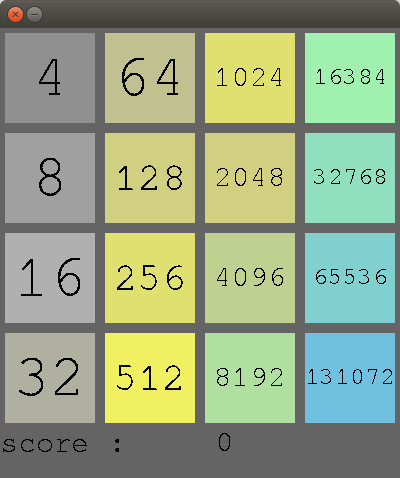
\includegraphics[scale = 0.5]{2048.png}

\end{document}